% +------------------------------------------------------------------------+
% | Reference manual page: Triangulation_utils_3.tex
% +------------------------------------------------------------------------+
% | 27.3.2000   Monique Teillaud
% | Package: Triangulation3
% | 
\RCSdef{\RCSTriangulationutilsRev}{$Revision$}
\RCSdefDate{\RCSTriangulationutilsDate}{$Date$}
% |
%%RefPage: end of header, begin of main body
% +------------------------------------------------------------------------+


\begin{ccRefClass}{Triangulation_utils_3}  %% add template arg's if necessary

%% \ccHtmlCrossLink{}     %% add further rules for cross referencing links
%% \ccHtmlIndexC[class]{} %% add further index entries

\ccDefinition
  
The class \ccRefName\ defines operations on the indices of vertices
and neighbors within a cell. These operations are used in
\ccc{Triangulation_3.h},
\ccc{Triangulation_data_structure_3.h},
\ccc{Triangulation_ds_cell_3.h},
\ccc{Triangulation_ds_circulators_3.h}. These classes inherit from
\ccRefName\ so that they can use its methods.

\ccInclude{CGAL/Triangulation_utils_3.h}

\ccThree{unsigned int}{ccw(unsigned int i)toto}{}

\ccFunction{unsigned int next_around_edge(unsigned int i, 
				    unsigned int j) const;}
{In dimension~3, index of the neighbor \ccc{n} that is next to the current cell,
when turning positively around an oriented edge whose endpoints are
indexed \ccc{i} and \ccc{j}. According to the usual numbering of
vertices and neighbors in a given cell, it is also the index of the vertex 
opposite to this neighbor \ccc{n}. (see Figure~\ref{Triangulation3-fig-utils}).
\ccPrecond{\ccc{( i < 4 ) && ( j < 4 ) && ( i != j )}.}}

\ccFunction{unsigned int ccw(unsigned int i) const;}
{Has a meaning only in dimension~2.\\
 Computes the index of the vertex that is next to the vertex numbered
\ccc{i} in counterclockwise direction. (see
Figure~\ref{Triangulation3-fig-utils}).  
\ccPrecond{\ccc{i<3}.}}

\ccFunction{unsigned int cw(unsigned int i) const;}
{Same for clockwise.}

\begin{figure}[htbp]
\begin{ccTexOnly}
\begin{center} 
\includegraphics{utils.eps} 
\end{center}
\end{ccTexOnly}
\caption{Operations on indices.
\label{Triangulation3-fig-utils}}
\begin{ccHtmlOnly}
<CENTER>
<img border=0 src="./utils.gif" align=center alt="Operations on indices">
</CENTER>
\end{ccHtmlOnly}
\end{figure} 



%% \ccExample

%% \ccIncludeExampleCode{examples/Triangulation3/Triangulation_utils_3_prog.C}

\end{ccRefClass}

% +------------------------------------------------------------------------+
%%RefPage: end of main body, begin of footer
% EOF
% +------------------------------------------------------------------------+

